\documentclass[../../ASSD_TP1_G7.tex]{subfiles}
\begin{document}
\chapter*{Sample and hold}
El amplificador \textit{sample-and-hold}, o SHA, mantiene el valor de una se\~nal anal\'ogica por un determinado tiempo. Es frecuentemente utilizado para conversiones anal\'ogico-digital. Se utiliza el circuito integrado $LF398$. Por consigna, $FS = 2\cdot 5V = 10V$.
\[\frac{1}{2}\text{LSB} = 0.5\cdot \frac{FS}{2^8} = \frac{10V}{2^9} \approx 20mV\]


\section{Especificaciones de se\~nales de entrada y alimentaci\'on}
\begin{itemize}
	\item Siguiendo las recomendaciones del fabricante, se utiliza alimentaci\'on partida de $\pm 15V$.
	\item El cambio entre el modo \textit{sample} y el modo \textit{hold} est\'a controlado por la se\~nal \textit{LOGIC REFERENCE} (conectada a tierra), y \textit{LOGIC}, proveniente del oscilador. \todo{insertar referencia a la secci\'on del oscilador} Si \textit{LOGIC - LOGIC REFERENCE} > 2.4V, se encuentra en modo \textit{sample}. En caso contrario, se encuentra en modo \textit{hold}.
	\item La se\~nal anal\'ogica de entrada, o \textit{input}, tiene una amplitud m\'axima de 5V por consigna y una m\'imina XXXXXXXX kHz debido a las limitaciones de rango din\'amico del filtro. \todo{Completar con rango dinamico del filtro}
\end{itemize}

\section{Fuentes de error}
\begin{itemize}
	\item \textbf{Retardos:}
	\begin{itemize}
		\item \textbf{Retardo de la se\~nal digital:} (El siguiente an\'alisis desprecia el retardo en la se\~nal anal\'ogica producido por el buffer de entrada). Si la se\~nal \textit{LOGIC} cambia de modo \textit{sample} a \textit{hold} en el instante $t_0$, debido a que \'esta tiene un retardo de $\Delta t_D$, la se\~nal de salida en el modo \textit{hold} ser\'a la correspondiente a la entrada anal\'ogica en $t_0 + \Delta t_D$ y no en $t_0$, tal como se esperar\'ia en un modelo ideal. Este an\'alisis desprecia el retardo en la se\~nal anal\'ogica al pasar por el buffer de entrada.
		\item \textbf{Retardo en la se\~nal anal\'ogica:} (El siguiente an\'alisis desprecia el retardo en la se\~nal \textit{LOGIC}). El buffer de entrada introduce un retraso $\Delta t_A(f)$ en la se\~nal de entrada. En consecuencia, al pasar del modo \textit{sample} al modo \textit{hold} en el instante $t_0$, la salida  ser\'a la correspondiente a la entrada  en $t_0 - \Delta t_A(f)$ y no en $t_0$.
	\end{itemize}
	\todo{de donde saco el ancho de banda?}
	Uniendo los dos puntos anteriores, si \textit{LOGIC} cambia a modo \textit{hold} en $t_0$, la salida ser\'a la correspondiente a la entrada en el instante $t_0 + \Delta t_D - \Delta t_A(f)$ (considerando ideal todos los dem\'as aspectos del sistema).
	
	\item \textbf{Tensi\'on de offset ($V_{OS})$:}
	
	$V_{OS}$ debe ser menor que $\frac{1}{2}$LSB = $20mV$ para que la conversi\'on anal\'ogico a digital sea precisa.  
	El valor t\'ipico especificado por el fabricante es $V_{OS} = 1mV$, valor por debajo de $\frac{1}{2}$LSB. Por este motivo, se considera innecesario el uso de un circuito que compense $V_{OS}$. 
\end{itemize}


\section{Elecci\'on del capacitor}
\subsection{Capacidad}
Consideraciones:
\begin{itemize}
	\item \textbf{Hold step:}
	Es el escal\'on de tensi\'on generado por transferencia de carga hacia el capacitor $C_H$ al cambiar de \textit{sample} a \textit{hold}. Siendo $V_H$ la altura del escal\'on, y $Q$ la carga que se transfiere al capacitor, se obtiene: \todo{La carga que se transfiere al capacitor est\'a relacionada con la capacidad par\'asita de la llave??}
	\[V_H = \frac{Q}{C_H}\]
	De esta relaci\'on se obtiene que para reducir el \textit{hold step} es necesario aumentar $C_H$.

		\begin{figure}[H]
			\centering
			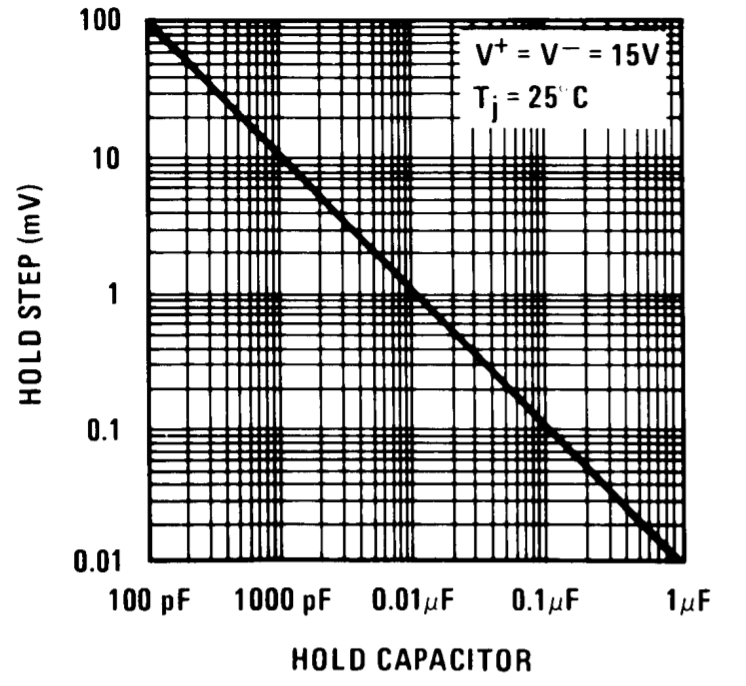
\includegraphics[width = 0.5\textwidth]{figures/hold_step_datasheet.png}
			\caption{Hold step en funci\'on de $C_H$.}
			\label{fig:syh_hold_step_datasheet}
		\end{figure}

Al igual que $V_{OS}$, el hold step $V_{HS}$ tiene que ser menor que $\frac{1}{2} LSB$ = $20mV$. Dejando un m\'argen de seguridad, se limita el valor de $V_{HS}$ a $10mV$ o menos, de forma que \[ C_H \geqslant 1nF \]
	
	
	\item\textbf{Acquisition time}
	
Como la resolucion es de 8bits, el error debe ser menor que $\frac{1}{2}$LSB = $\frac{FS}{2^9} = FS \cdot 0.02\% $. Por lo tanto, se utiliza la curva de 0.01\% de la hoja de datos (figura \ref{fig:syh_acquisition_time_datasheet}).

Frecuencia de sampleo: $f_s = 100kHZ $ \\
Periodo de sampleo: $T_s = \frac{1}{f_s} = 10\mu s$


El sistema tiene $10\mu s$ para estar en modo \textit{sample} y en modo \textit{hold}, por lo que el tiempo de adquisici\'on hasta 0.2\% debe ser menor a $10\mu s$. De lo contrario no tendr\'ia tiempo para estar en modo sample. De la curva de 0.1\% de la figura \ref{fig:syh_acquisition_time_datasheet} se observa que para que se cumplan los requisitos anteriores se debe cumplor que \[C_H \leqslant 4nF\]

 
		\begin{figure}[H]
			\centering
			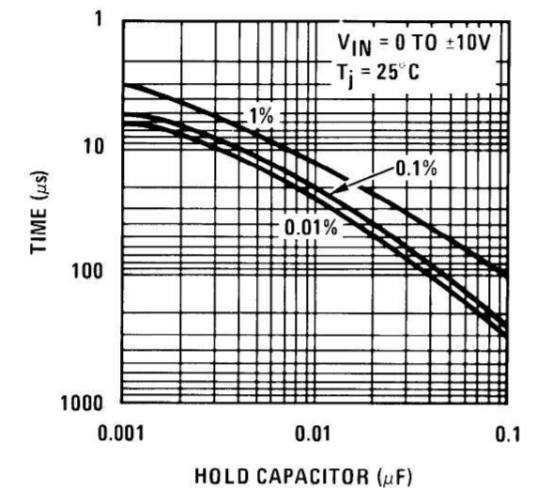
\includegraphics[width = 0.5\textwidth]{figures/acquisition_time_datasheet.png}
			\caption{Tiempo de adquisici\'on en funci\'on de $C_H$.}
			\label{fig:syh_acquisition_time_datasheet}
		\end{figure}	
		
		
		
	\item \textbf{Droop rate}
	
	El droop rate no presenta una limitaci\'on para esta aplicaci\'on en particular debido a los cortos tiempos de hold con los que se trabaja. Suponiendo que su valor es el m\'aximo presentado por el fabricante ($1V/s$), como el tiempo de \textit{hold} es menor que $10\mu s$, el m\'aximo error posible por \textit{droop} es $10\mu V$, lo cual es despreciable frente a $\frac{1}{2}$LSB = $10mV$.1
	
		\begin{figure}[H]
			\centering
			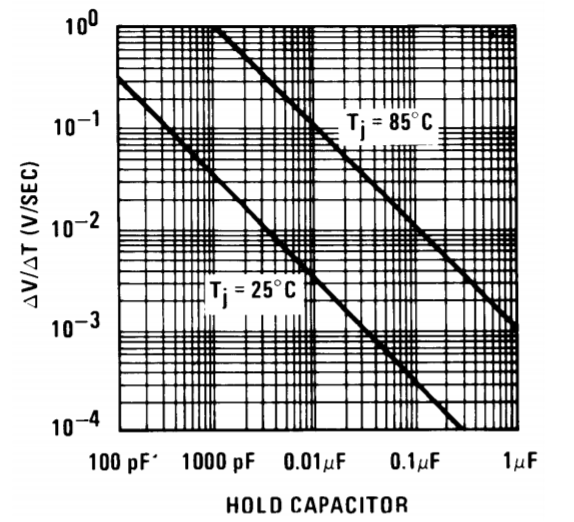
\includegraphics[width = 0.5\textwidth]{figures/droop_datasheet.png}
			\caption{Droop rate en funci\'on de $C_H$.}
		\end{figure}	
\end{itemize}

Adem\'as de las restricciones anteriores, es importante considerar que si existiera el ADC, ser\'ia conveniente que el tiempo de \textit{sample} sea lo m\'as chico posible comparado con el tiempo de \textit{hold}. Por lo tanto, se prioriza acortar lo m\'as posible el tiempo de adquisici\'on: \[C_H=1nF\]

\subsection{Tecnolog\'ia}
Uno con baja absorcion dielectrica.


\section{Duty cycle}
Se elige un duty cycle de 50\%, lo cual deja $5 \mu s$ para el modo \textit{sample} y $5 \mu s$ para el modo hold. Hay tiempo suficiente como para que se establezca la se\~nal en el modo \textit{sample} al menos al 0.1\% (con que se establezca al 0.2\% alcanzar\'ia para un ADC 8 bits). En la figura \ref{fig:syh_hold_settling_time_datasheet} se observa que el tiempo de establecimiento en modo \textit{hold} es menor a $1.4\mu s$ para el rango de temperaturas posibles de trabajo, por lo que quedar\'ian $5\mu s - 1.4 \mu s = 3.6 \mu s$ de se\~nal lo suficientemente establecida como para ser sampleada por un ADC.

		\begin{figure}[H]
			\centering
			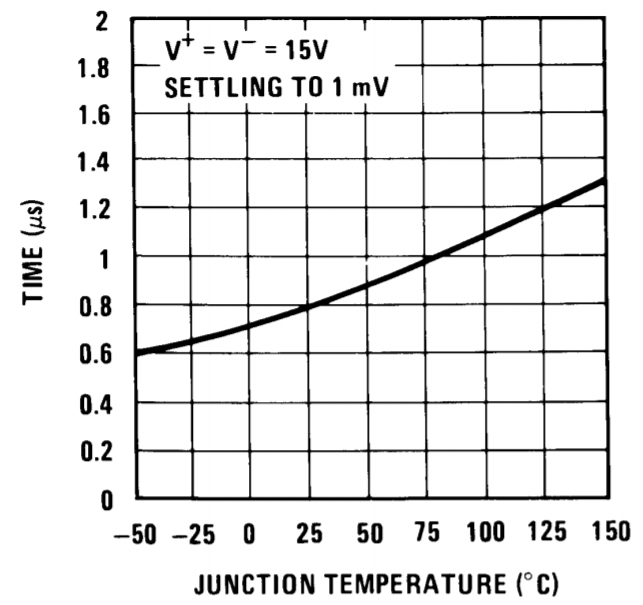
\includegraphics[width = 0.5\textwidth]{figures/hold_settling_time_datasheet.png}
			\caption{Hold settling time en funci\'on de la temperatura.}
			\label{fig:syh_hold_settling_time_datasheet}
		\end{figure}


\section{Circuito de correcci\'on de offset} \label{sec:syh_correccion_offset}

		\begin{figure}[H]
			\centering
			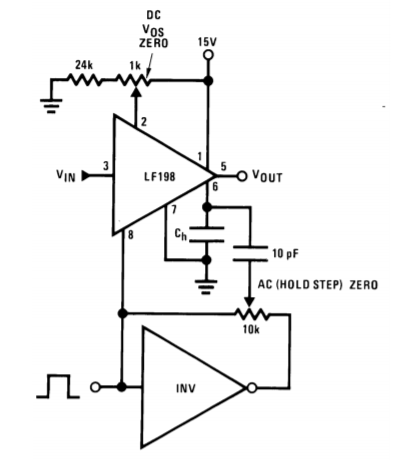
\includegraphics[width = 0.5\textwidth]{figures/offset_adjust_schematic.png}
			\caption{Circuito de correcci\'on de \textit{hold step} y de tensi\'on de offset $V_{OS}$.}
			\label{fig:syh_offset_correction_datasheet}
		\end{figure}	
		

\section{Mediciones}

\begin{figure}[H]
	\centering
	\begin{tikzpicture}
\begin{axis}[
	xlabel = Tiempo (s),
	ylabel = Tensi\'on (V),
	width = \textwidth, 
	cycle list name = color list,
	ytick = {-5,...,5}]
\addplot table [x=x-axis, y=1, col sep=comma] {\pgfpath../mediciones/sh_1m2_2m4_n.csv};
\addplot table [x=x-axis, y=2, col sep=comma] {\pgfpath../mediciones/sh_1m2_2m4_n.csv};
\addplot table [x=x-axis, y=3, col sep=comma] {\pgfpath../mediciones/sh_1m2_2m4_n.csv};
\addplot table [x=x-axis, y=4, col sep=comma] {\pgfpath../mediciones/sh_1m2_2m4_n.csv};

\legend{Input, Output, Tensi\'on $C_H$, SCSH}
\end{axis}
\end{tikzpicture}
	\caption{Medici\'on \textit{sample and hold}. $f_{entrada} = 1M2$, $f_{SCSH}=2M4$, $C_H = 100nF$.}
\end{figure}

\begin{figure}[H]
	\centering
	\input{figures/syh_8k3_20k_100n.tikz}
	\caption{Medici\'on \textit{sample and hold}. $f_{entrada} = 8K3$, $f_{SCSH}=20K$, $C_H = 100nF$.}
\end{figure}

\begin{figure}[H]
	\centering
	\input{figures/syh_8k3_20k_100n_sim.tikz}
	\caption{Simulaci\'on \textit{sample and hold}. $f_{entrada} = 8K3$, $f_{SCSH}=20K$, $C_H = 100nF$.}
\end{figure}


\begin{figure}[H]
	\centering
	\begin{tikzpicture}
\begin{axis}[
	xlabel = Tiempo (s),
	ylabel = Tensi\'on (V),
	width = \textwidth, 
	cycle list name = color list,
	ytick = {-4,...,5},
	ymax = 3.5
	]
\addplot table [x=x-axis, y=1, col sep=comma] {\pgfpath../mediciones/sh_1m2_2m4_p.csv};
\addplot table [x=x-axis, y=2, col sep=comma] {\pgfpath../mediciones/sh_1m2_2m4_p.csv};
\addplot table [x=x-axis, y=3, col sep=comma] {\pgfpath../mediciones/sh_1m2_2m4_p.csv};
\addplot table [x=x-axis, y=4, col sep=comma] {\pgfpath../mediciones/sh_1m2_2m4_p.csv};

\legend{Input, Output, Tensi\'on $C_H$, SCSH}
\end{axis}
\end{tikzpicture}
	\caption{Medici\'on \textit{sample and hold}. $f_{entrada} = 1M2$, $f_{SCSH}=2M4$, $C_H = 100pF$.}
\end{figure}

\begin{figure}[H]
	\centering
	\input{figures/syh_8k3_20k_100p.tikz}
	\caption{Medici\'on \textit{sample and hold}. $f_{entrada} = 8K3$, $f_{SCSH}=20K$, $C_H = 100pF$.}
\end{figure}

\begin{figure}[H]
	\centering
	\input{figures/syh_8k3_20k_100p_zoom.tikz}
	\caption{Detalle de la medici\'on \textit{sample and hold}. $f_{entrada} = 8K3$, $f_{SCSH}=20K$, $C_H = 100pF$.}
\end{figure}

\end{document}
